% =====================================================================
%  A COMPLETE, EXPLAINED MANUSCRIPT
%  Per-site retrieval of lunar regolith thermal conductivity K_d at the
%  Apollo 15 & 17 heat-flow boreholes: the physics, the code, and the method,
%  from the ground up. Merges the teaching guidebook and the method write-up.
%
%  Self-contained for Overleaf: upload this folder (manuscript.tex + figures/).
%  Compile:  latexmk -pdf manuscript.tex
% =====================================================================
\documentclass[11pt]{report}

\usepackage[a4paper,margin=2.4cm]{geometry}
\setlength{\emergencystretch}{3em}
\usepackage[T1]{fontenc}
\usepackage{newtxtext,newtxmath}
\usepackage[scaled=0.90]{helvet}
\usepackage{microtype}
\usepackage{amsmath}
\usepackage{graphicx}
\usepackage{booktabs}
\usepackage{array}
\usepackage{xcolor}
\usepackage{listings}
\usepackage[most]{tcolorbox}
\usepackage{enumitem}
\usepackage{titlesec}
\usepackage{fancyhdr}
\usepackage[hidelinks]{hyperref}

% ---- palette ----
\definecolor{forest}{HTML}{3D6E4A}
\definecolor{coral}{HTML}{B85B3A}
\definecolor{teal}{HTML}{2C6E73}
\definecolor{char}{HTML}{2B2B2B}
\definecolor{dim}{HTML}{6B6B6B}
\definecolor{rulec}{HTML}{C9C2B6}
\definecolor{codebg}{HTML}{F4F2EE}
\definecolor{codekw}{HTML}{3D6E4A}
\definecolor{codestr}{HTML}{B85B3A}
\hypersetup{colorlinks=true,allcolors=teal}

% ---- headings ----
\titleformat{\chapter}[display]{\normalfont\sffamily\huge\bfseries\color{forest}}
  {\sffamily\large\color{dim}Chapter \thechapter}{2pt}{\Huge}
\titleformat{\section}{\normalfont\sffamily\large\bfseries\color{forest}}{\thesection}{0.6em}{}
\titleformat{\subsection}{\normalfont\sffamily\bfseries\color{char}}{\thesubsection}{0.5em}{}
\titlespacing*{\chapter}{0pt}{6pt}{14pt}

\pagestyle{fancy}\fancyhf{}
\renewcommand{\headrulewidth}{0.4pt}
\fancyhead[L]{\sffamily\footnotesize\color{dim}Apollo $K_d$ --- complete manuscript}
\fancyhead[R]{\sffamily\footnotesize\color{dim}\thepage}

% ---- code listings ----
\lstdefinestyle{py}{language=Python, basicstyle=\ttfamily\footnotesize\color{char},
  backgroundcolor=\color{codebg}, frame=single, framerule=0pt, rulecolor=\color{rulec},
  keywordstyle=\color{codekw}\bfseries, commentstyle=\color{dim}\itshape,
  stringstyle=\color{codestr}, showstringspaces=false, breaklines=true,
  columns=fullflexible, xleftmargin=8pt, aboveskip=7pt, belowskip=4pt,
  literate={->}{{$\rightarrow$}}2 {**}{{$^{\wedge}$}}1}

\newcommand{\Tm}{\langle T\rangle}
\newcommand{\code}[1]{{\ttfamily\small #1}}

% ---- callout boxes ----
\newtcolorbox{plain}[1][]{colback=teal!6,colframe=teal!55,boxrule=0.6pt,arc=2pt,
  left=8pt,right=8pt,top=4pt,bottom=4pt,
  title={\sffamily\bfseries In plain words},coltitle=teal,fonttitle=\small,#1}
\newtcolorbox{talk}[1][]{colback=coral!8,colframe=coral!70,boxrule=1pt,arc=2pt,
  left=8pt,right=8pt,top=4pt,bottom=4pt,
  title={\sffamily\bfseries $\bigstar$\ \ FOR TOMORROW'S TALK},coltitle=coral,fonttitle=\small,#1}
\newtcolorbox{keypt}[1][]{colback=forest!7,colframe=forest!55,boxrule=0.7pt,arc=2pt,
  left=8pt,right=8pt,top=4pt,bottom=4pt,
  title={\sffamily\bfseries Key point},coltitle=forest,fonttitle=\small,#1}

\begin{document}

% ================= TITLE =================
\thispagestyle{empty}
\begingroup\color{forest}\hrule height 2.5pt\endgroup
\vspace{14pt}
{\sffamily\bfseries\color{forest}\LARGE Per-site retrieval of lunar regolith\\[3pt]
thermal conductivity $K_d$ at the Apollo 15 \& 17\\[3pt]
heat-flow boreholes\par}
\vspace{10pt}
{\sffamily\Large\color{char} The physics, the code, and the method --- explained from the ground up\par}
\vspace{12pt}
{\color{dim}\large A complete companion manuscript to the JGR letter.\par}
\vspace{6pt}
{\color{char} R.\,P.\ Gregorio \quad\textbullet\quad Kasai Laboratory, Institute of Science Tokyo}
\vspace{8pt}
\begingroup\color{rulec}\hrule height 1pt\endgroup
\vspace{16pt}

\begin{abstract}
\noindent
We measure how well heat conducts through the deep lunar regolith --- the
parameter $K_d$ --- separately at the Apollo~15 and Apollo~17 heat-flow
boreholes, and find them to differ by about a factor of two
($K_{d,\mathrm{A15}}^{*}=4.58$, $K_{d,\mathrm{A17}}^{*}=8.12$
mW\,m$^{-1}$\,K$^{-1}$). This document explains \emph{everything} behind that
sentence, assuming no prior knowledge: what heat conduction is and how we model
it; the two published conductivity models and how to reproduce them; the
numerical solver line by line; the subtle bug we found in reaching steady state
and the faster, self-certifying method that replaced it; how $K_d$ is actually
retrieved from the data; how the uncertainty is quantified; why the basal heat
flux $Q_b$ matters; and why the two sites plausibly differ. Figures and code
listings accompany every step. Sections needed for the oral presentation are
marked with a $\bigstar$.
\end{abstract}

\vspace{6pt}
\begin{talk}
\textbf{If you only prepare a few things, prepare these (each is one slide):}
\begin{enumerate}[leftmargin=1.4em,itemsep=1pt,topsep=2pt]
\item The question \& the two sites --- \S\ref{sec:question}, Fig.~\ref{fig:map}.
\item What $K_d$ is and the conductivity models --- \S\ref{sec:hayne}, Fig.~\ref{fig:models}.
\item Why we need steady state --- \S\ref{sec:whyss}.
\item Old vs.\ new solver (the GIFs) --- \S\ref{sec:oldnew}, Figs.~\ref{fig:spinfilm},~\ref{fig:newfilm}.
\item They give the same answer --- \S\ref{sec:agree}, Fig.~\ref{fig:overlay}.
\item The retrieval \& the result --- \S\ref{sec:retrieval}, Figs.~\ref{fig:sweep},~\ref{fig:profiles}.
\item $K_d$ depends on $Q_b$ --- \S\ref{sec:qb}, Fig.~\ref{fig:qb}.
\item Why the sites differ --- \S\ref{sec:sites}.
\end{enumerate}
\end{talk}

\clearpage
\tableofcontents
\clearpage

% =====================================================================
\chapter{What we are trying to do, and why}\label{ch:intro}
% =====================================================================
\section{The question}\label{sec:question}
Every airless body loses its internal heat through a blanket of broken rock ---
\emph{regolith}. How fast that heat escapes, and how steeply temperature rises
with depth, is controlled by the regolith's \textbf{thermal conductivity}: a
number, $K$, that says how many watts of heat flow through a square metre for
each degree of temperature change per metre of depth (units
W\,m$^{-1}$\,K$^{-1}$). Deep down, that number settles to a value we call
$K_d$ (``$d$'' for deep).

The Apollo~15 and~17 missions buried temperature probes in the Moon (the
Heat-Flow Experiment, HFE) and recorded subsurface temperatures from 1971 to
1977. The standard practice is to assume \emph{one} global $K_d$ for the whole
Moon. \textbf{Our question is simply: what is $K_d$ at each of the two boreholes,
separately --- and do they differ?} (Fig.~\ref{fig:map}.)

\begin{figure}[h]\centering
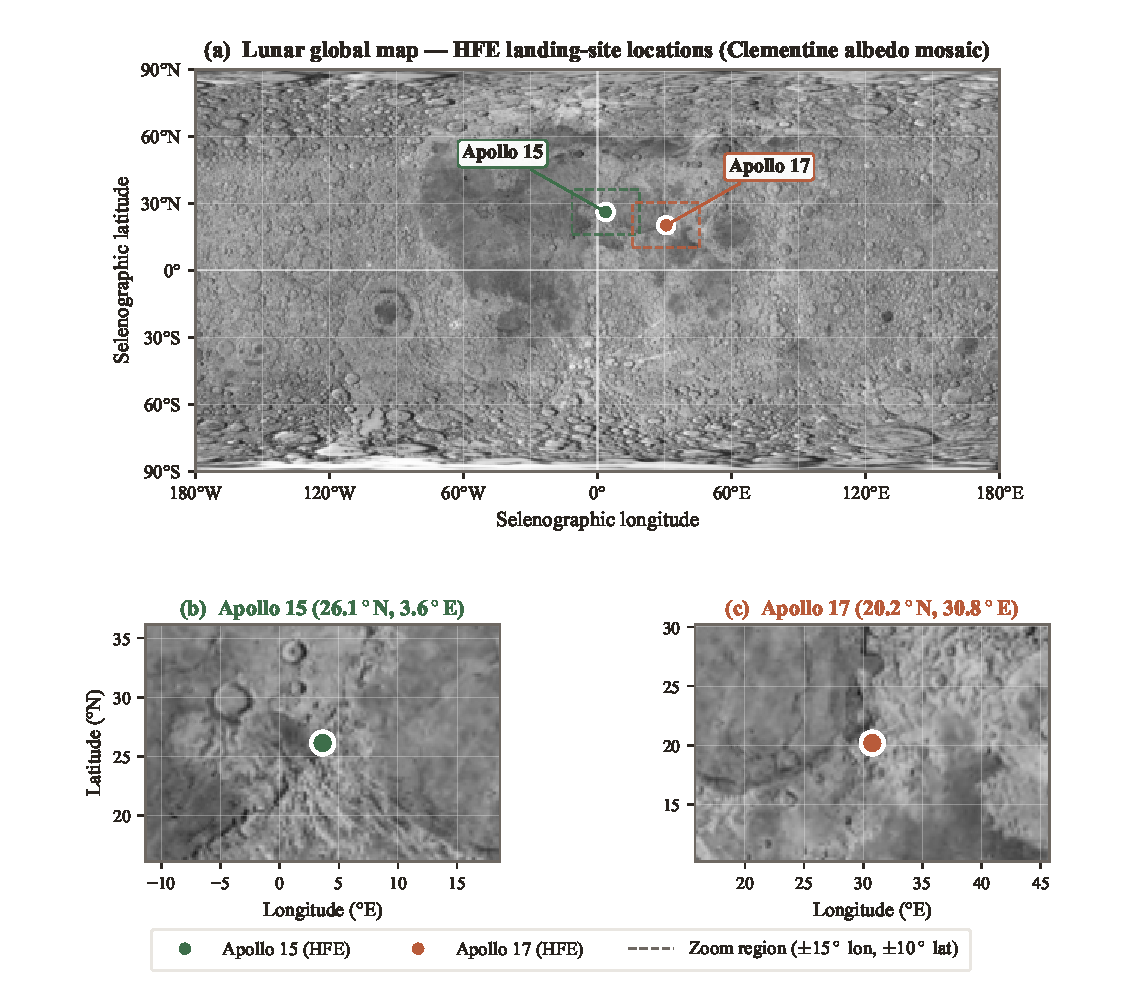
\includegraphics[width=0.7\linewidth]{figures/fig_context_map.pdf}
\caption{The two heat-flow boreholes. Apollo~15 sits at Hadley Rille on the
Imbrium mare/Apennine boundary; Apollo~17 in the Taurus--Littrow highland valley.
Different terrains $\rightarrow$ possibly different regolith.}
\label{fig:map}
\end{figure}

\section{Why it matters}
$K_d$ sets the deep temperature, which feeds models of subsurface ice stability,
future drilling and habitat thermal design, and the Moon's heat budget. A wrong,
one-size-fits-all $K_d$ propagates into all of them. Getting it right \emph{per
site} is the contribution.

\section{The shape of the whole argument}
In one breath: \emph{(i)} heat conduction is described by one equation; \emph{(ii)}
two published formulas give $K$ as a function of temperature and depth; \emph{(iii)}
we put one of them in a computer model of the regolith and run it until it stops
changing (``steady state''); \emph{(iv)} we ask which $K_d$ makes the model's deep
temperatures match the Apollo sensors; \emph{(v)} the hard part was reaching
steady state correctly --- the bulk of this document --- and \emph{(vi)} we then
quantify the uncertainty and interpret the result. Each clause is a chapter.

% =====================================================================
\chapter{The physics, from the ground up}\label{ch:physics}
% =====================================================================
\section{Heat conduction and the heat equation}
Heat flows from hot to cold. Fourier's law says the heat flux $q$
(W\,m$^{-2}$) through a material is proportional to how steeply temperature
changes with position:
\begin{equation}
q = -K\,\frac{\partial T}{\partial z},
\label{eq:fourier}
\end{equation}
where $z$ is depth and $K$ the conductivity. The minus sign says heat flows
\emph{downhill} in temperature. Now demand energy conservation in a thin slab:
the rate at which it stores heat equals what flows in minus what flows out.
That gives the \textbf{heat equation},
\begin{equation}
\rho(z)\,c_p(T)\,\frac{\partial T}{\partial t}
   = \frac{\partial}{\partial z}\!\left(K(T,z)\,\frac{\partial T}{\partial z}\right),
\label{eq:heat}
\end{equation}
where $\rho$ is density (kg\,m$^{-3}$) and $c_p$ the specific heat
(J\,kg$^{-1}$\,K$^{-1}$): the left side is ``heat stored,'' the right side is
``net heat conducted in.'' This single equation is the physics of the entire
study (Fig.~\ref{fig:conduction}).

\begin{figure}[h]\centering
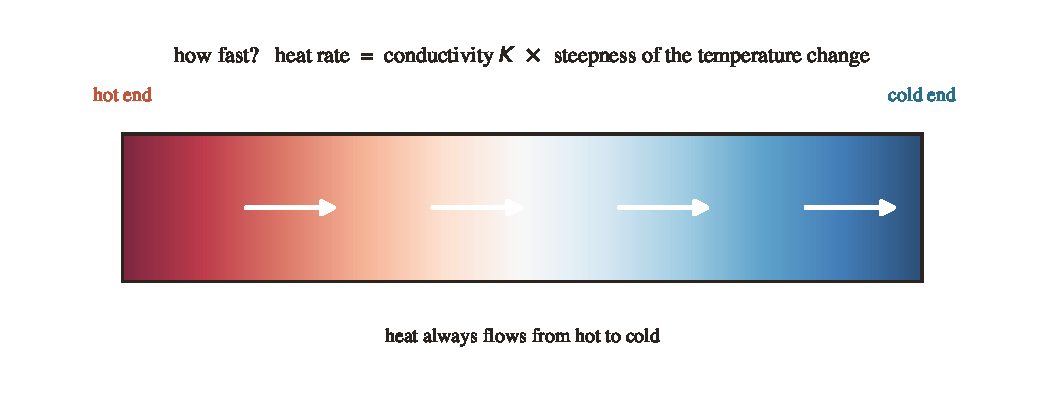
\includegraphics[width=0.82\linewidth]{figures/fig_book_conduction.pdf}
\caption{Heat conduction in a column: flux $q=-K\,\partial_z T$ moves heat down
the temperature gradient; the heat equation is the bookkeeping of what each
layer stores versus passes on.}
\label{fig:conduction}
\end{figure}

\begin{plain}
Think of the regolith as a stack of thin layers. Each layer can hold heat
(that's $\rho c_p$) and can pass heat to its neighbours (that's $K$). The heat
equation just says: a layer warms up if more heat arrives than leaves. Solving it
means tracking that exchange through time and depth.
\end{plain}

\section{The lunar forcing: the daily wave and the skin depth}
At the surface, the Sun drives a huge day--night temperature swing (from
$\sim$100\,K at night to $\sim$390\,K at noon). This ``thermal wave'' travels
downward but \emph{dies out} quickly: its amplitude falls by $1/e$ over the
\textbf{skin depth} $\delta=\sqrt{2\kappa/\omega}$, where $\kappa=K/(\rho c_p)$ is
the thermal diffusivity and $\omega=2\pi/P$ the angular frequency of the lunar
day. For the Moon $\delta\approx10$--$20$\,cm. Below a few skin depths, the
regolith barely feels day or night --- it responds only to the \emph{average}
heating. This split (a fast, shallow daily wave on top of a slow, deep mean) is
the single most important fact for everything that follows.

\section{Boundary conditions: top and bottom}
Equation~\eqref{eq:heat} needs a rule at each end of the column.
\begin{itemize}[leftmargin=1.4em,itemsep=2pt]
\item \textbf{Top (surface): a radiative energy balance.} The surface has no
contact with anything above it, so sunlight absorbed must equal heat radiated
away plus heat conducted down:
\begin{equation}
(1-A)\,S(t) = \varepsilon\sigma T_s^4 + K\,\frac{\partial T}{\partial z}\Big|_{0},
\label{eq:surfbc}
\end{equation}
with $A$ the albedo (reflectivity), $S(t)$ the incident sunlight, $\varepsilon$
the emissivity, and $\sigma$ the Stefan--Boltzmann constant. The $T_s^4$ makes
this \emph{non-linear} --- it must be solved numerically each timestep.
\item \textbf{Bottom: the geothermal flux.} From far below, the Moon's interior
supplies a small, steady heat flux $Q_b$ (about $15$--$21$\,mW\,m$^{-2}$). So at
the base of the column, $K\,\partial_z T = Q_b$.
\end{itemize}

\section{Periodic steady state and flux closure}\label{sec:fluxclosure}
After long enough, the column reaches a \textbf{periodic steady state}: every
lunation is identical to the last. Two conditions define it, and we will lean on
the second one constantly:
\begin{enumerate}[leftmargin=1.5em,itemsep=2pt]
\item the surface skin repeats its daily cycle;
\item below the skin there are no heat sources, so in steady state the same
geothermal flux passes through \emph{every} layer. With Fourier's law this fixes
the deep gradient of the cycle-mean temperature $\Tm$:
\begin{equation}
\boxed{\;K(\Tm,z)\,\frac{d\Tm}{dz}=Q_b
\quad\Longrightarrow\quad
\frac{d\Tm}{dz}=\frac{Q_b}{K(\Tm,z)}\;}
\label{eq:closure}
\end{equation}
\end{enumerate}

\begin{keypt}
Equation~\eqref{eq:closure} is the backbone of the whole method. It says the deep
temperature profile is \emph{not} a free thing to be discovered --- once you know
the temperature at one depth, energy conservation fixes the slope everywhere
below. Remember it; Chapters~\ref{ch:steady} and~\ref{ch:retrieval} are built on
it.
\end{keypt}

% =====================================================================
\chapter{The two conductivity models (and how to reproduce them)}\label{ch:models}
% =====================================================================
$K$ is not a single number --- it depends on temperature (hotter regolith
radiates across pores, conducting better) and depth (deeper regolith is
compacted, conducting better). Two published models capture this.

\section{Hayne et al.\ (2017): the H-parameter model}\label{sec:hayne}
The solid ``contact'' conductivity rises from a surface value $K_s$ to a deep
value $K_d$ as the regolith compacts, over an $e$-folding depth $H$; a radiative
term $\propto T^3$ is added on top:
\begin{align}
K_c(z) &= K_d - (K_d-K_s)\,e^{-z/H}, \label{eq:Kc}\\
K(T,z) &= K_c(z)\,\bigl[\,1+\chi\,(T/T_{\mathrm{ref}})^3\,\bigr].\label{eq:Khayne}
\end{align}
In code this is four lines (\code{lunar/properties.py}):
\begin{lstlisting}[style=py]
def conductivity_hayne(T, z, Ks=7.4e-4, Kd=3.4e-3, H=0.06, chi=2.7):
    Kc = Kd - (Kd - Ks) * np.exp(-z / H)          # contact part: K_s -> K_d
    return Kc * (1.0 + chi * (T / 350.0) ** 3)    # + radiative T^3 term
\end{lstlisting}
The published parameters: $K_s=0.74$, $K_d=3.4$ mW\,m$^{-1}$\,K$^{-1}$;
$H=6$\,cm; $\chi=2.7$; $T_{\mathrm{ref}}=350$\,K. The density follows the same
shape, $\rho(z)=\rho_d-(\rho_d-\rho_s)e^{-z/H}$ with $\rho_s=1100$,
$\rho_d=1800$ kg\,m$^{-3}$.

\paragraph{Why the literature $K_d$ is $3.4$.} Hayne et al.\ fit
Eqs.~\eqref{eq:Kc}--\eqref{eq:Khayne} to the \emph{globally averaged} day--night
temperature curves measured from orbit by the Diviner instrument. A single set of
parameters reproduced the global average, and $K_d=3.4$ is that global deep
asymptote. It was never site-specific --- which is the gap we fill
(Fig.~\ref{fig:models}a).

\section{Mart\'inez \& Siegler (2021): a density-based model}
This writes $K$ directly in terms of bulk density $\rho$:
\begin{equation}
K(T,\rho)=(A_1\rho+A_2)\,k_{\mathrm{am}}(T)+(B_1\rho+B_2)\,T^3,
\label{eq:Kmartinez}
\end{equation}
with $k_{\mathrm{am}}(T)$ a fitted amorphous-solid polynomial. Same idea, different
knobs: where Hayne's free parameter is $K_d$, Mart\'inez's is effectively the deep
density. We use it as an independent cross-check (Ch.~\ref{ch:crosschecks}).

\begin{figure}[h]\centering

\includegraphics[width=\linewidth]{figures/fig_models.pdf}
\caption{(a) Hayne contact conductivity $K_c(z)$: it rises from $K_s$ to its deep
asymptote $K_d$. The published global value is $3.4$; our retrievals move it to
$4.58$ (A15) and $8.12$ (A17). (b) Full $K(T)$ at 1\,m for both models --- the
radiative term roughly doubles $K$ by midday.}
\label{fig:models}
\end{figure}

% =====================================================================
\chapter{The numerical solver, line by line}\label{ch:solver}
% =====================================================================
We cannot solve Eq.~\eqref{eq:heat} by hand, so we discretise: chop the column
into cells and time into steps, and advance the temperature numerically
(Fig.~\ref{fig:numerical}).

\begin{figure}[h]\centering
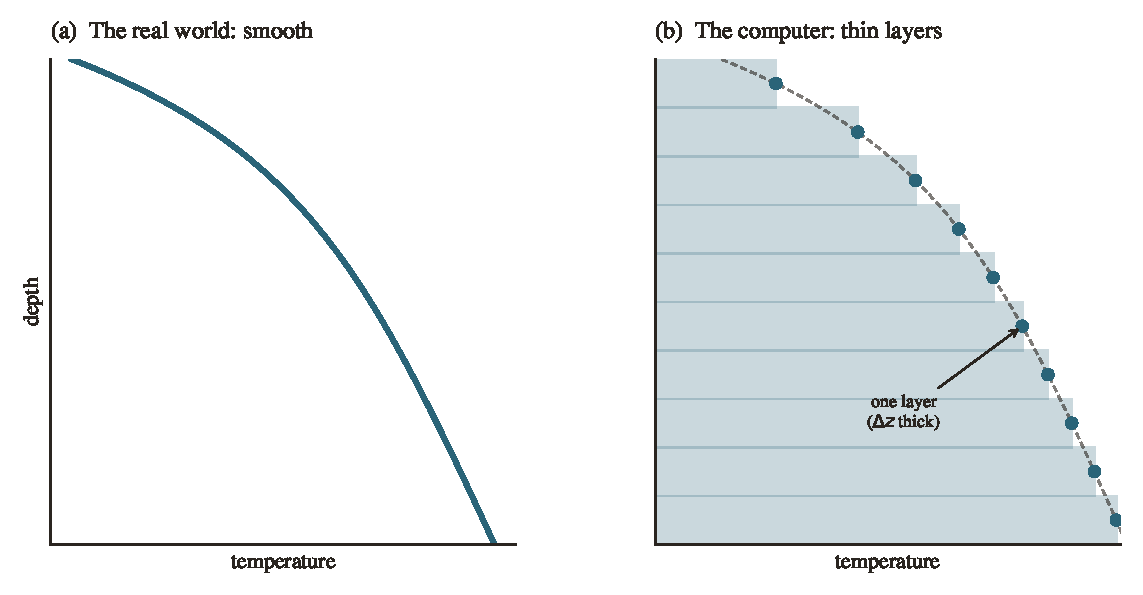
\includegraphics[width=0.82\linewidth]{figures/fig_book_numerical.pdf}
\caption{Discretising the column: cells in depth, steps in time; each step solves
a small linear system that couples each cell to its neighbours.}
\label{fig:numerical}
\end{figure}

\section{The geometric depth grid}
The daily wave needs millimetre resolution at the top, but the deep column can be
coarse. So the cells grow geometrically with depth --- each $\sim$8\% thicker
than the one above:
\begin{lstlisting}[style=py]
def make_geometric_grid(z_max=5.0, dz0=0.002, growth=0.08):
    faces, dz = [0.0], dz0
    while faces[-1] < z_max:
        faces.append(faces[-1] + dz)
        dz *= (1 + growth)              # each layer ~8% thicker
    # cell centres z_mid, thicknesses dz follow from the faces
\end{lstlisting}
This gives $\sim$69 cells: fine where it matters, cheap where it does not.

\section{One time step: Crank--Nicolson}
We use the Crank--Nicolson scheme (second-order accurate, unconditionally
stable). It averages the heat flow at the old and new time levels, producing a
tridiagonal linear system $A\,T^{n+1}=d$ for the new temperatures. With
face conductances $\alpha^{L}_i,\alpha^{R}_i$ (from harmonic-mean face
conductivities and the cell heat capacity $c_i=\rho_i c_{p,i}\Delta z_i$):
\begin{lstlisting}[style=py]
K   = K_func(T_prev, z_mid)              # conductivity at current T
Kf  = harmonic_mean(K)                   # conductivity at cell faces
cap = rho * cp_func(T_prev) * dz         # heat capacity of each cell
aL  = dt * Kf[:-1] / (dz_c[:-1] * cap)   # left-face conductance
aR  = dt * Kf[1:]  / (dz_c[1:]  * cap)   # right-face conductance
a = -0.5*aL;  c = -0.5*aR;  b = 1 + 0.5*(aL + aR)        # the matrix A
d = 0.5*aL*Tleft + (1 - 0.5*(aL+aR))*T_prev + 0.5*aR*Tright   # the RHS
\end{lstlisting}
(Full version: \code{lunar/solver.py}, function \code{\_step}.)

\section{Solving the system: the Thomas algorithm}
A tridiagonal system is solved in one downward sweep and one upward sweep ---
fast and exact:
\begin{lstlisting}[style=py]
for i in range(1, n):                    # forward elimination
    m     = b[i] - a[i]*cp[i-1]
    cp[i] = c[i] / m
    dp[i] = (d[i] - a[i]*dp[i-1]) / m
x[n-1] = dp[n-1]
for i in range(n-2, -1, -1):             # back-substitution
    x[i] = dp[i] - cp[i]*x[i+1]
\end{lstlisting}

\section{The non-linear surface: Newton's method}
The surface energy balance Eq.~\eqref{eq:surfbc} has a $T_s^4$, so we cannot solve
for $T_s$ directly. We use Newton's method: guess $T_s$, compute how far the
balance is from zero ($R$), and its slope ($R'$), and step:
\begin{lstlisting}[style=py]
for _ in range(max_iter):
    R  = (1-A)*S - eps*sigma*Ts**4 - Ksurf*(Ts - Tsub)/(0.5*dz0)
    dR = -4*eps*sigma*Ts**3 - 2*Ksurf/dz0
    Ts = Ts - R/dR                       # Newton update; converges in a few steps
\end{lstlisting}

\section{Stepping through a lunation: the spin-up loop}
To find the steady state the brute-force way, we step through one lunation
($\sim$709 hourly steps), compare to the previous lunation, and repeat:
\begin{lstlisting}[style=py]
for cycle in range(1, n_lunations_spinup + 1):
    T_start = T.copy()
    for k in range(1, n_t):              # march through one lunar day
        T = step(T, ...)
    if max(abs(T - T_start)) < 0.01 and cycle >= 2:
        break                            # "converged"  <-- the trap (see Ch.5)
\end{lstlisting}
This works --- but \emph{how many} lunations is the whole problem of the next
chapter.

% =====================================================================
\chapter{Reaching steady state: the old method, the bug, and the fix}\label{ch:steady}
% =====================================================================

\section{Why we even need steady state}\label{sec:whyss}
We compare modelled deep temperatures to the Apollo sensors. The sensors recorded
a \emph{settled} regolith (we keep only the late, stable part of the record). And
$K_d$ is a \emph{steady-state property}: its fingerprint is the settled deep
gradient $d\Tm/dz=Q_b/K_d$ (Eq.~\eqref{eq:closure}) --- a gentler slope for higher
$K_d$. Before the model settles, its deep gradient is still forming and reflects
the starting guess, not $K_d$. So we can only read $K_d$ off a settled profile.

\begin{plain}
Judging $K_d$ from an un-settled model is like judging how well a wall insulates
by watching the temperature across it \emph{while it is still warming up}: the
slope is changing for reasons that have nothing to do with the insulation. You
must wait for it to steady --- or compute the steady state directly.
\end{plain}

\section{The old method and the bug we found (flag F1)}\label{sec:oldnew}
The original code reached steady state by a \emph{fixed} 30-lunation spin-up
(\S\ref{ch:solver}). \textbf{The symptom of trouble:} the retrieved $K_d$ changed
when we changed the starting temperature --- a physical answer must not. The
diagnosis: the column relaxes on the diffusive timescale of its full depth,
\begin{equation}
\tau\sim z_{\max}^2/\kappa\approx \text{order }10^3\ \text{lunations},
\end{equation}
so after 30 lunations the deep regolith still holds its initial value
(Fig.~\ref{fig:spinfilm}). Worse, the convergence test \emph{lied}: because the
deep drift is so slow, the cycle-to-cycle change is already $<0.01$\,K while the
profile is far from settled. The sensors at $0.8$--$2.4$\,m sit exactly in the
unsettled zone, so the starting guess leaked straight into $K_d$.

\begin{figure}[h]\centering
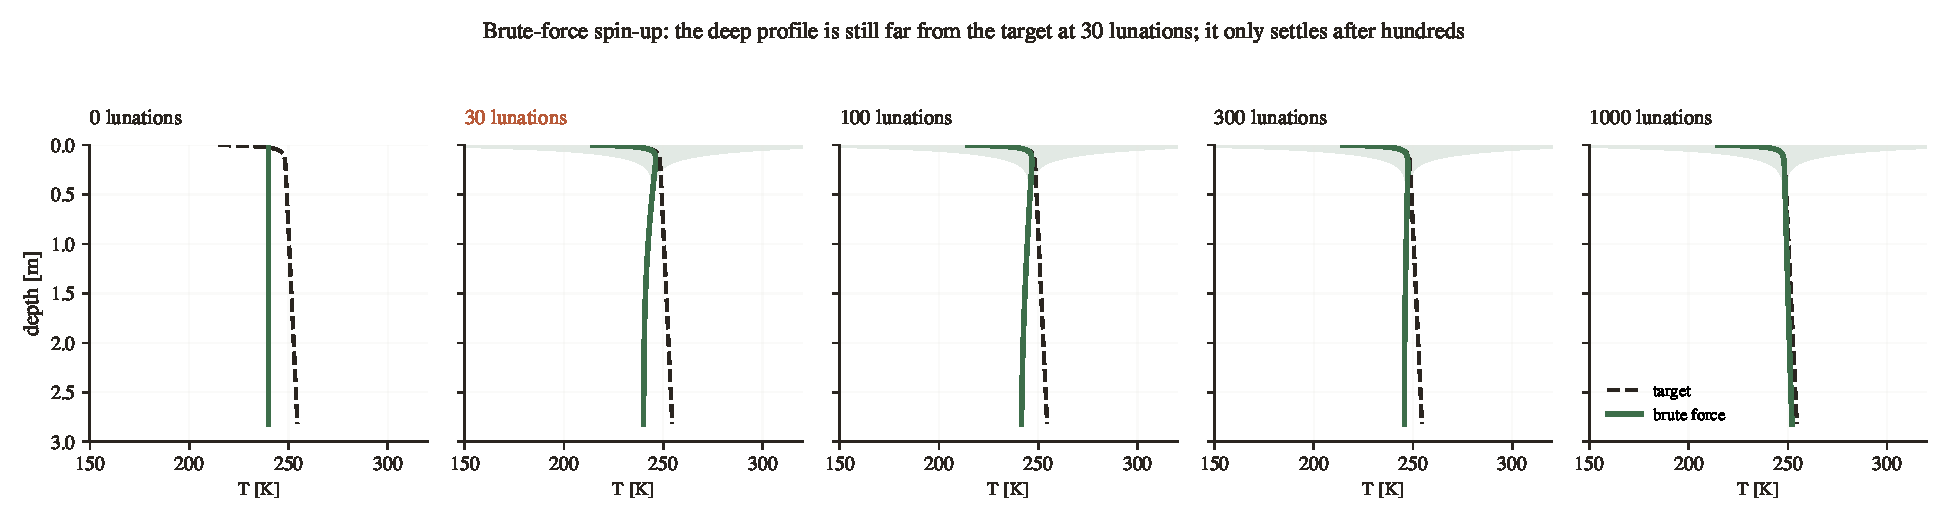
\includegraphics[width=\linewidth]{figures/spinup_filmstrip.pdf}
\caption{The old method (animated in \code{spinup.gif}). Green $=$ current
profile, dashed $=$ true steady state, shaded $=$ daily swing. At 30 lunations
only the top $\sim$0.5\,m has moved; the deep part still sits at the start. It
takes hundreds of lunations to settle.}
\label{fig:spinfilm}
\end{figure}

\begin{talk}
This is the crux of the ``what went wrong'' story. Show \code{spinup.gif}: the
heat visibly fails to reach the deep sensors in 30 lunations, so the old $K_d$
was biased by the starting guess. One sentence: \emph{``a fixed short spin-up
never settles the deep regolith, so the answer depended on where we started.''}
\end{talk}

\section{The fix: a flux-anchored shortcut}
The escape is to use Eq.~\eqref{eq:closure} instead of waiting for it. The new
solver alternates two moves (Fig.~\ref{fig:newfilm}, animated in
\code{newmethod.gif}):
\begin{description}[leftmargin=2.4em,itemsep=2pt]
\item[Step A --- settle the skin.] A \emph{short} spin-up (a few lunations)
settles only the fast surface skin and reads the cycle-mean ``anchor''
temperature just below it.
\item[Step B --- reconstruct the deep profile.] From the anchor, integrate
$d\Tm/dz=Q_b/K$ straight down. This \emph{computes} the deep profile in one shot
instead of waiting for heat to diffuse there.
\end{description}
The reconstruction is the surprising part --- the deep temperatures are not
simulated, they are walked out from the anchor along the known slope:
\begin{lstlisting}[style=py]
for i in range(i0, N-1):                 # walk downward from the anchor depth
    q   = Q_b - u[i]                     # u = small rectification correction
    Ki  = K(T[i], z[i])
    Th  = T[i] + 0.5*q/Ki*dz             # midpoint (RK2) for accuracy
    T[i+1] = T[i] + q/K(Th, z_half)*dz   # dT/dz = (Q_b - u)/K
\end{lstlisting}
With $Q_b=21$\,mW\,m$^{-2}$ and $K\approx9$\,mW\,m$^{-1}$\,K$^{-1}$ at depth, the
slope is $\sim$2.3\,K/m, so each metre below the anchor adds $\sim$2.3\,K
(animated in \code{reconstruct.gif}).

\begin{figure}[h]\centering
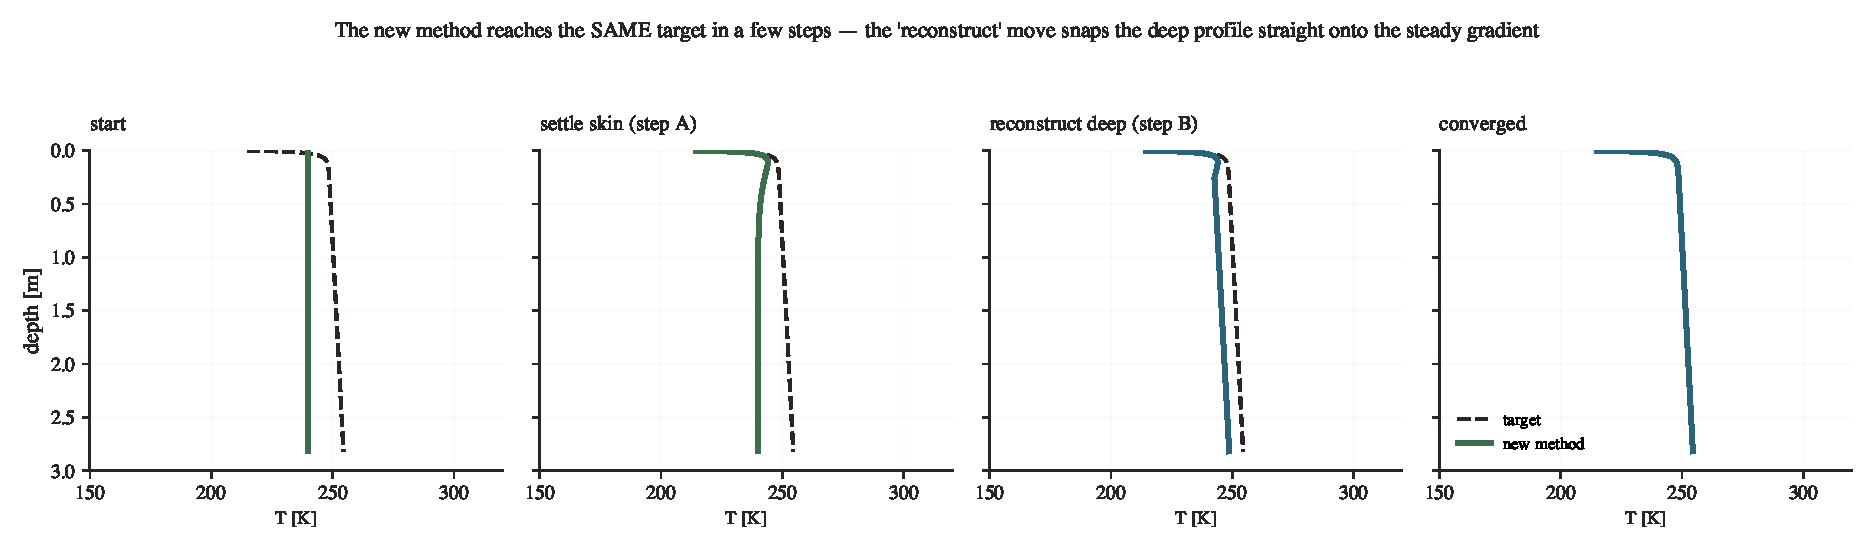
\includegraphics[width=\linewidth]{figures/newmethod_filmstrip.pdf}
\caption{The new method (animated in \code{newmethod.gif}). Step A settles the
skin; Step B's reconstruct move snaps the deep profile onto the steady gradient;
a dozen short rounds refine it to the target.}
\label{fig:newfilm}
\end{figure}

The two moves are iterated in a short two-stage loop:
\begin{lstlisting}[style=py]
for stage in (coarse_anchor_0.25m, fine_anchor_0.55m):
    for it in range(stage.max_iters):
        out = solve_pixel(..., n_lunations_spinup=stage.n_inner)  # Step A
        Tm  = out.T.mean(axis=1)                                  # cycle mean
        u   = rectified_flux(out.T, z, K)
        T   = reconstruct(Tm, z, stage.anchor, Q_b, K, u)         # Step B
        if abs(Tm[anchor] - prev) < stage.tol and it >= 2: break  # drift check
        prev = Tm[anchor]
\end{lstlisting}
In total this uses $\sim$150 lunations of stepping ($\sim$9\,s), versus the
$\sim$1000+ lunations the old method must crawl through.

\section{They give the same answer}\label{sec:agree}
The decisive check: take the \emph{old} method and just run it longer. As the
lunations increase, its profile marches onto the new method's answer
(Fig.~\ref{fig:conv}); started from two very different temperatures (240\,K and
260\,K) it lands on the same curve (Fig.~\ref{fig:overlay}). They must --- both
enforce the same two steady-state conditions, and the solution is unique. The new
method just reaches it without waiting.

\begin{figure}[h]\centering
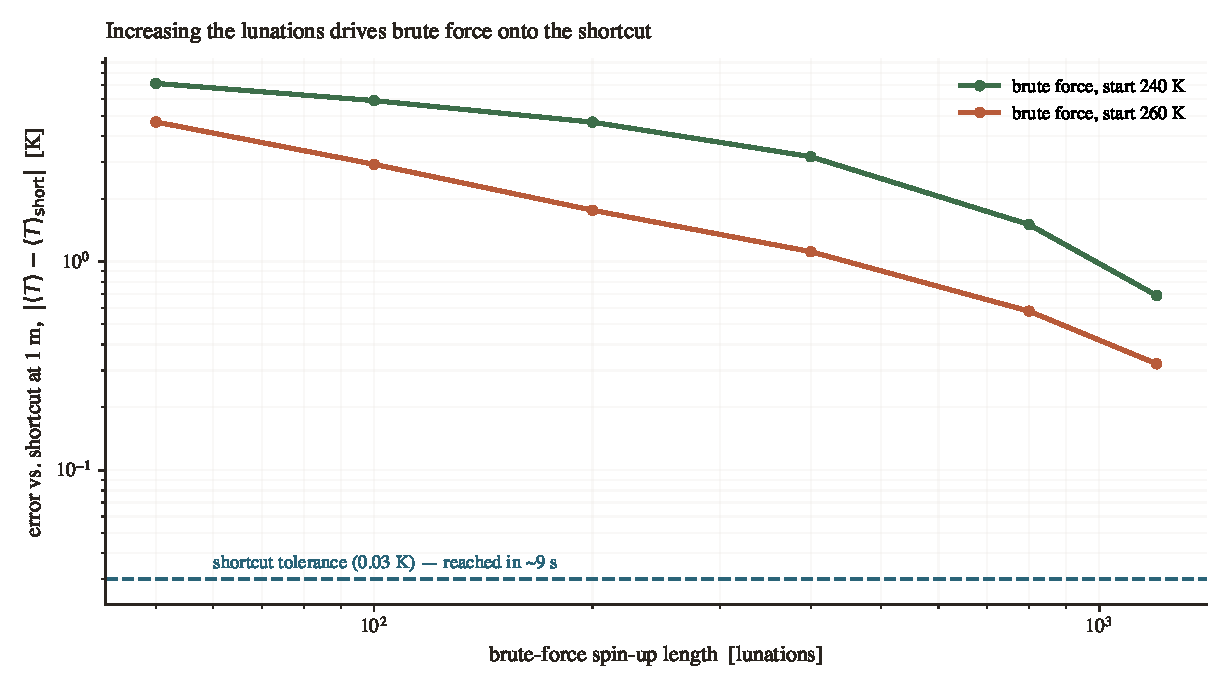
\includegraphics[width=0.66\linewidth]{figures/fig_convergence.pdf}
\caption{Brute-force error vs.\ the new method falls steadily as the spin-up
lengthens; two starts converge to the same value.}
\label{fig:conv}
\end{figure}
\begin{figure}[h]\centering
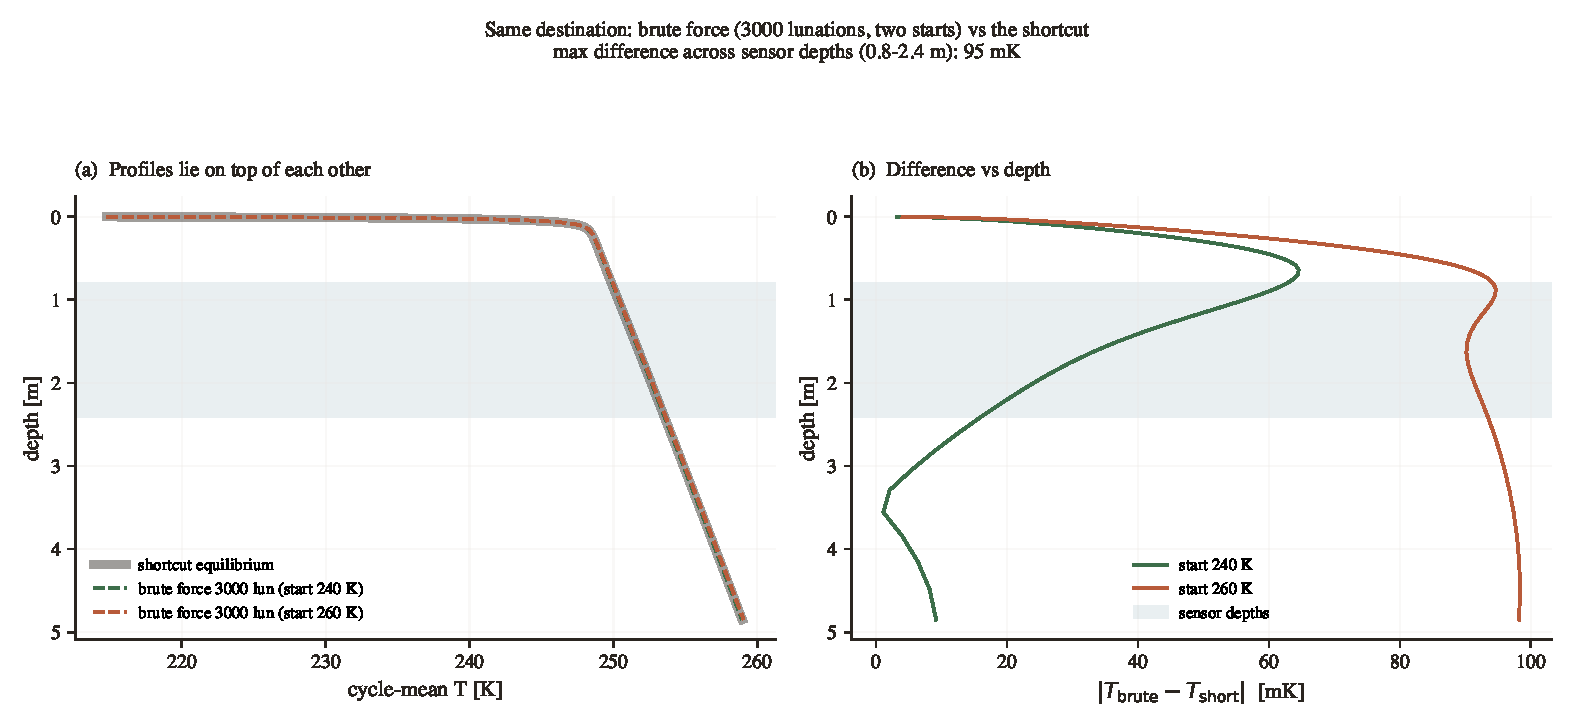
\includegraphics[width=\linewidth]{figures/fig_equilibrium_demo.pdf}
\caption{Brute force run to 3000 lunations from 240\,K and 260\,K (dashed) lies on
top of the new method (solid): same profile to tens of mK.}
\label{fig:overlay}
\end{figure}

\begin{talk}
The single most convincing slide. Two very different starting guesses, plus the
fast method, all land on one curve (Fig.~\ref{fig:overlay}). Say: \emph{``the new
method isn't a different model --- it reaches the exact same steady state, just
$\sim$30$\times$ faster, and it certifies that it got there.''}
\end{talk}

\section{It certifies itself}
Every solve returns two numbers proving convergence: the anchor \emph{drift}
between iterations ($<0.03$\,K; typically 3\,mK) and the \emph{flux closure}
$\max|\langle q\rangle-Q_b|/Q_b$ below the anchor ($<2\%$;
Fig.~\ref{fig:cert}). These are exactly the check the old fixed spin-up could
never pass.

\begin{figure}[h]\centering
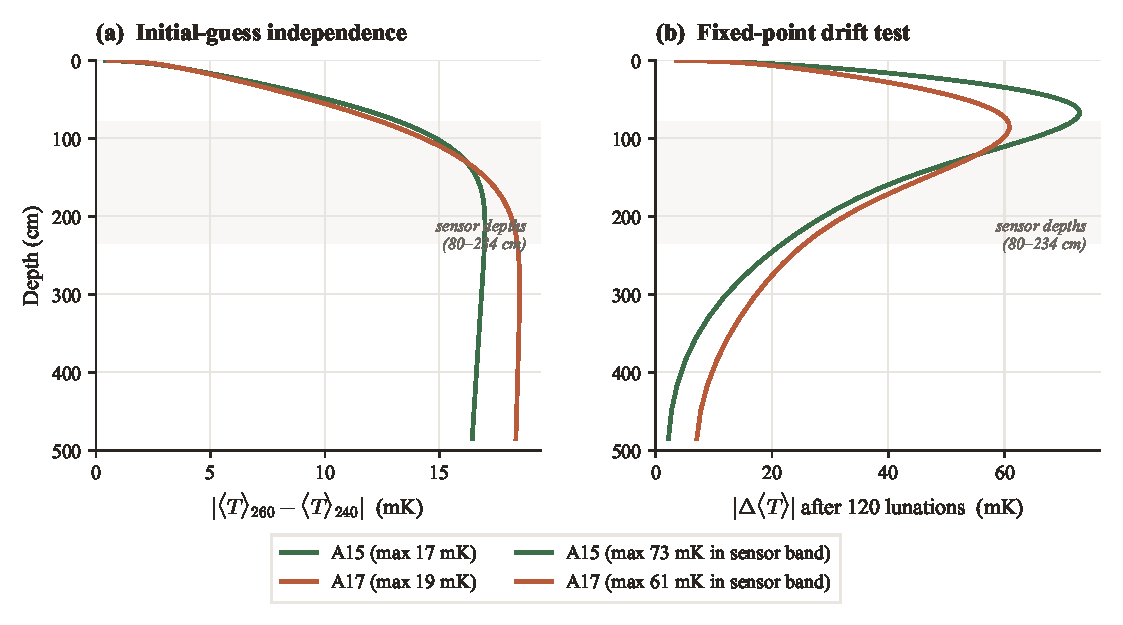
\includegraphics[width=0.78\linewidth]{figures/fig_equilibrium_certification.pdf}
\caption{Guess-independence and flux closure --- the returned proof that a solve
reached the steady state.}
\label{fig:cert}
\end{figure}

% =====================================================================
\chapter{Retrieving \texorpdfstring{$K_d$}{Kd} from the data}\label{ch:retrieval}\label{sec:retrieval}
% =====================================================================
\section{One forward run: \texttt{run\_with}}
The hub of the pipeline turns one trial $K_d$ into one settled profile:
\begin{lstlisting}[style=py]
def run_with(site, kd):
    grid  = make_geometric_grid(**GRID)
    insol = (1 - site.albedo) * S0 * solar_cosine(site)   # sunlight forcing
    K = lambda T, z: conductivity_hayne(T, z, Kd=kd)      # Hayne with this K_d
    eq = solve_periodic_equilibrium(grid, t, insol, Q_b=site.Q_b, K_func=K, ...)
    return grid.z_mid, eq.T_mean        # depths and the settled mean profile
\end{lstlisting}

\section{The sweep and the minimum}
We try a grid of $K_d$ values; for each, \code{run\_with} gives a settled profile,
and we measure the misfit to the deep sensors,
\begin{equation}
\mathrm{RMSE}(K_d)=\sqrt{\tfrac1N\textstyle\sum_i\bigl[\Tm(z_i;K_d)-T^{\rm obs}_i\bigr]^2}.
\end{equation}
The best-fit $K_d^{*}$ is the minimum, refined by fitting a parabola through the
three points around it:
\begin{lstlisting}[style=py]
rmse    = np.sqrt((R[idx]**2).mean(axis=0))     # RMSE at each trial K_d
k       = np.argmin(rmse)                        # nearest grid minimum
kd_star = parabola_vertex(kd_grid[k-1:k+2], rmse[k-1:k+2])   # sub-grid minimum
\end{lstlisting}
Each site shows a clean single minimum (Fig.~\ref{fig:sweep}).

\begin{figure}[h]\centering
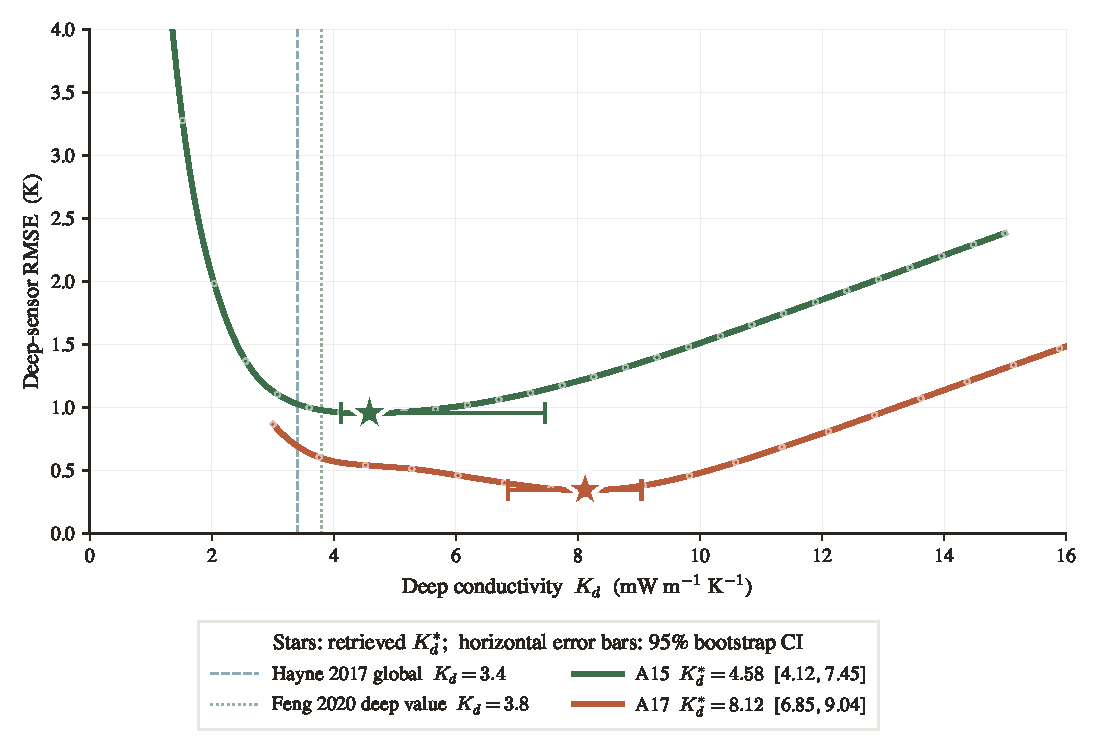
\includegraphics[width=0.74\linewidth]{figures/fig_kd_sweep.pdf}
\caption{Deep-sensor RMSE vs.\ trial $K_d$. The minimum is $K_d^{*}$; Apollo~17's
sits at a clearly higher conductivity than Apollo~15's.}
\label{fig:sweep}
\end{figure}

\section{The result}
\[
K_{d,\mathrm{A15}}^{*}=4.58,\qquad K_{d,\mathrm{A17}}^{*}=8.12\quad
\mathrm{mW\,m^{-1}\,K^{-1}},
\]
Apollo~17 about twice Apollo~15. With these the modelled deep temperatures track
the data far better than the global value (Fig.~\ref{fig:profiles}); at Apollo~17
the misfit roughly halves.

\begin{figure}[h]\centering
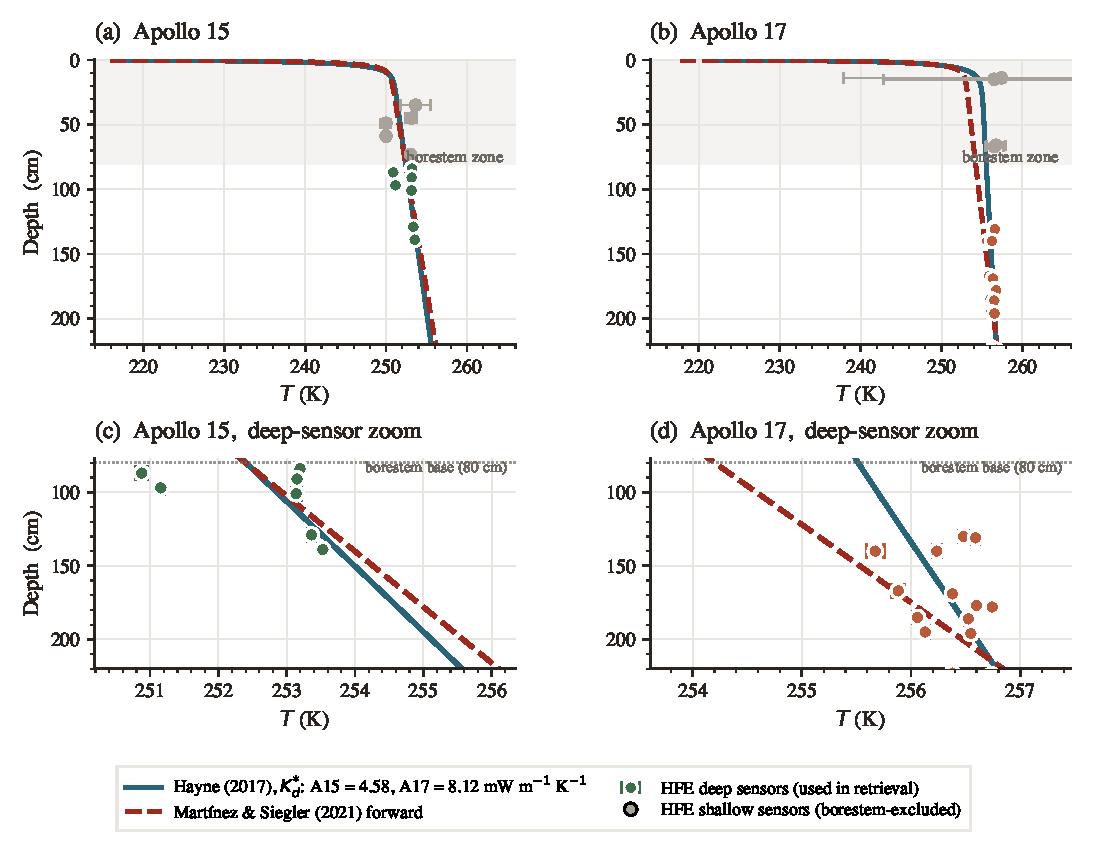
\includegraphics[width=0.74\linewidth]{figures/fig_thermal_profiles.pdf}
\caption{Settled mean temperature vs.\ depth using each site's retrieved
$K_d^{*}$, against the deep-sensor measurements.}
\label{fig:profiles}
\end{figure}

% =====================================================================
\chapter{How sure are we? (uncertainty)}\label{ch:stats}
% =====================================================================
\section{The bootstrap}
To get an error bar without assuming a noise model, we \emph{resample}: draw the
sensors with replacement (and jitter their depths by $\pm2.5$\,cm), re-fit
$K_d^{*}$, and repeat 1500 times. The spread of those 1500 fits is the
uncertainty (Fig.~\ref{fig:boot}). The 95\% intervals are
$[4.12,7.45]$ (A15) and $[6.85,9.04]$ (A17); the inter-site contrast is
$3.31$ with $p\approx0.011$ --- about a 1\% chance of being a fluke.

\begin{figure}[h]\centering
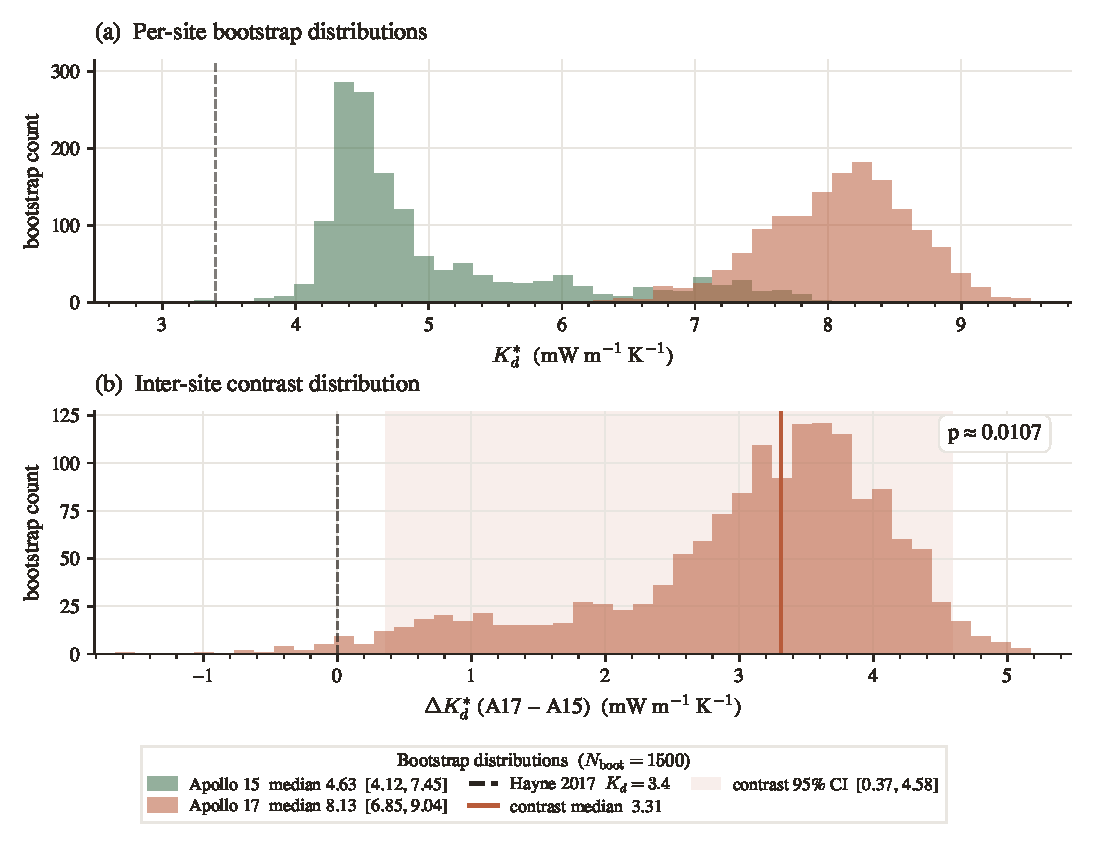
\includegraphics[width=0.92\linewidth]{figures/fig_bootstrap.pdf}
\caption{Bootstrap distributions of $K_d^{*}$. The two humps barely overlap ---
the contrast is statistically real.}
\label{fig:boot}
\end{figure}

\section{Bayesian cross-check and model selection}
An independent Bayesian sampler (Fig.~\ref{fig:mcmc} explains the idea) maps the
joint posterior in $(K_d,Q_b)$; even with $Q_b$ uncertain, Apollo~17 stays more
conductive $\sim$83\% of the time. A model comparison (AICc; Fig.~\ref{fig:aicc})
prefers ``different $K_d$ per site'' over ``one shared $K_d$'' --- so the data
favour a \emph{conductivity} contrast, not a flux artefact. (These are summarised
here; the letter carries the full treatment.)

\begin{figure}[h]\centering
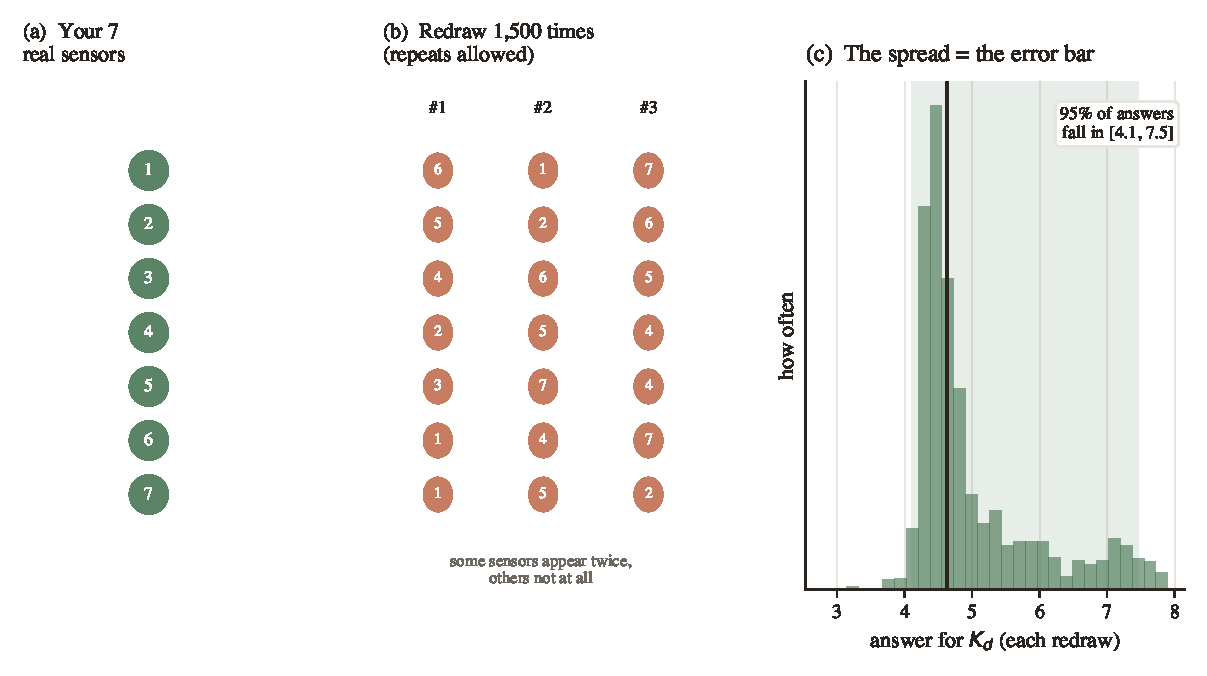
\includegraphics[width=0.74\linewidth]{figures/fig_book_bootstrap.pdf}
\caption{What the bootstrap does, schematically: resample the data many times,
re-fit each time, read the spread.}
\label{fig:bootschem}
\end{figure}
\begin{figure}[h]\centering
\begin{minipage}{0.49\linewidth}\centering
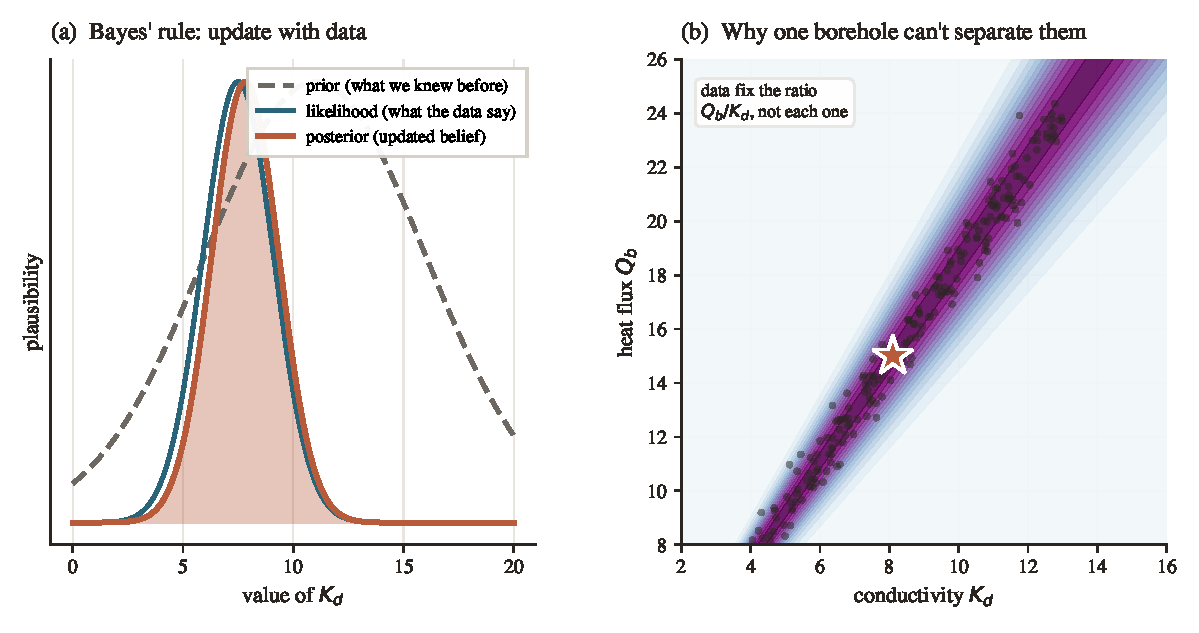
\includegraphics[width=\linewidth]{figures/fig_book_mcmc.pdf}\end{minipage}\hfill
\begin{minipage}{0.49\linewidth}\centering
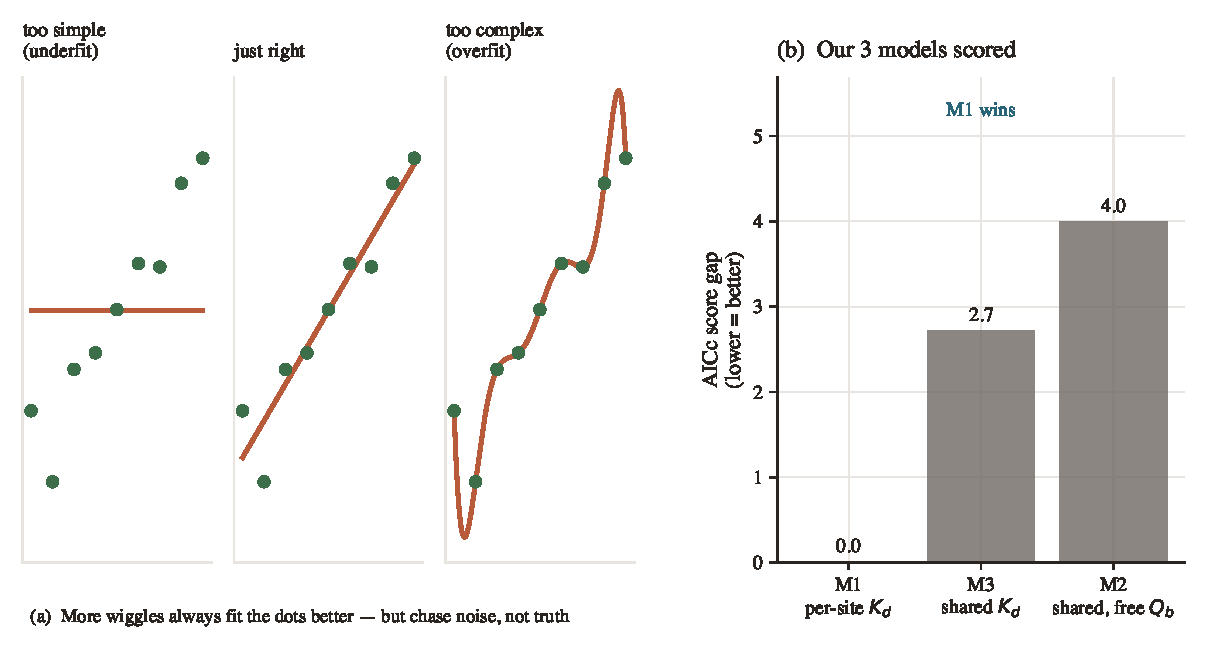
\includegraphics[width=\linewidth]{figures/fig_book_aicc.pdf}\end{minipage}
\caption{Left: the idea of MCMC posterior sampling. Right: AICc model selection
trades fit quality against the number of free parameters.}
\label{fig:mcmc}\label{fig:aicc}
\end{figure}

% =====================================================================
\chapter{The role of the basal flux \texorpdfstring{$Q_b$}{Qb}}\label{ch:qb}\label{sec:qb}
% =====================================================================
$K_d$ cannot be read in isolation. The deep gradient is $Q_b/K$
(Eq.~\eqref{eq:closure}), so $K_d$ and $Q_b$ trade off: assume more heat from
below and you infer a higher conductivity for the same temperatures
(Fig.~\ref{fig:qb}). This single record cannot separate them, so we \emph{fix}
$Q_b$ at the published values ($21$ and $15$\,mW\,m$^{-2}$) and report $K_d$
\emph{conditional} on them. The \emph{direction} of the contrast survives even
when $Q_b$ is allowed to vary, and $Q_b$ is one of the largest single terms in
the error budget --- a direct fingerprint of this coupling.

\begin{figure}[h]\centering
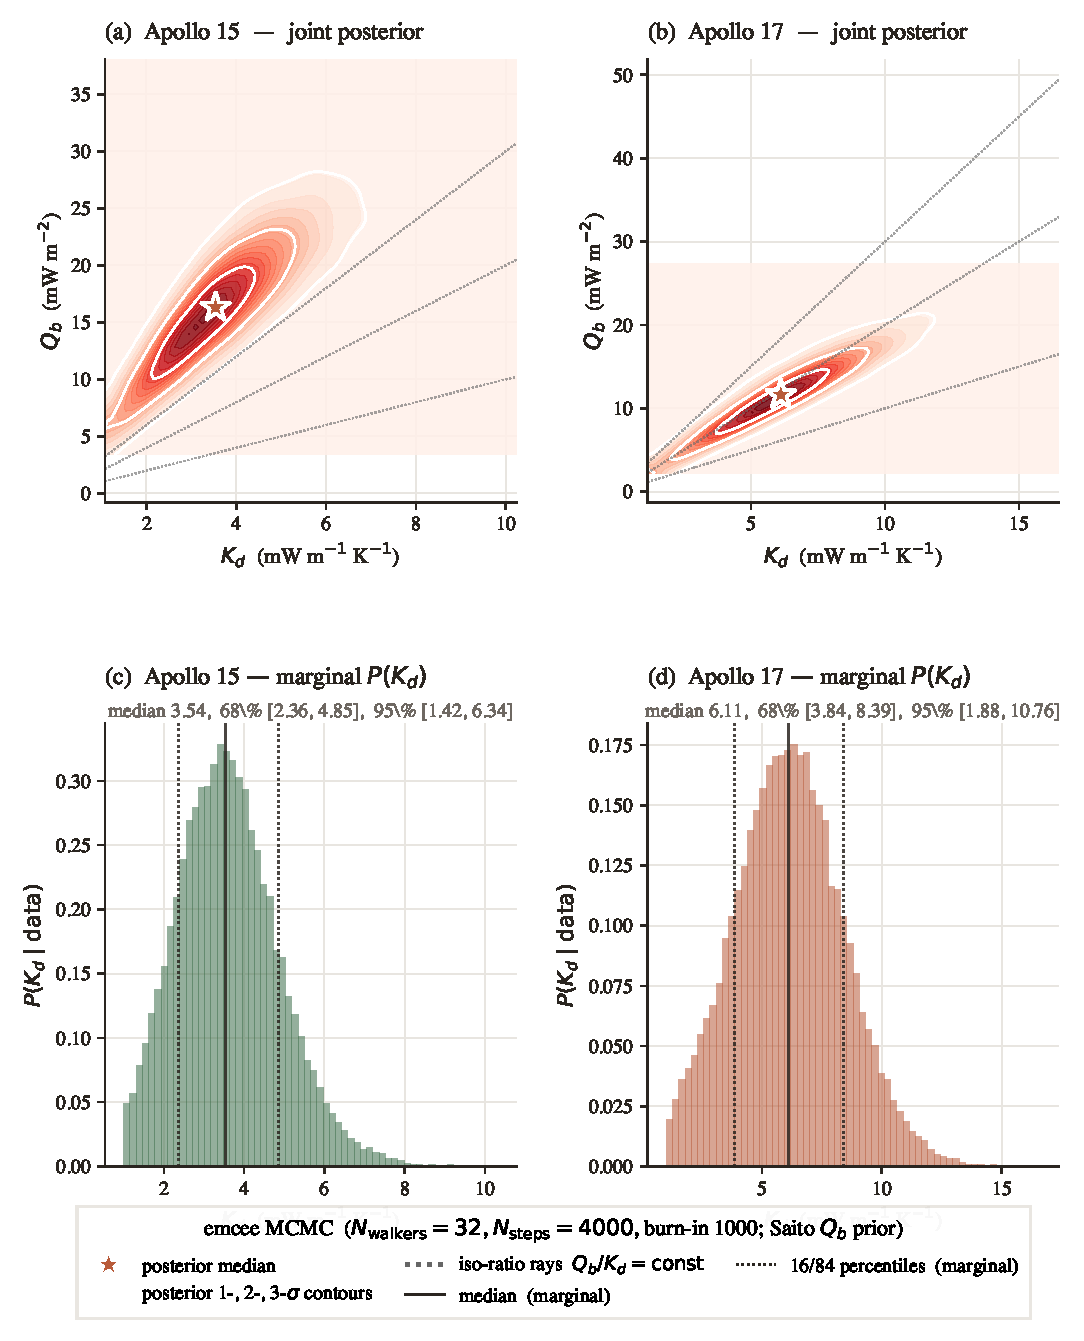
\includegraphics[width=0.6\linewidth]{figures/fig_kd_qb_posterior.pdf}
\caption{The $K_d$--$Q_b$ trade-off: many combinations along a diagonal fit
almost equally well, so $K_d$ is conditional on $Q_b$. The contrast between sites
is more robust than either absolute value.}
\label{fig:qb}
\end{figure}

\begin{talk}
Pre-empt the obvious question. Say up front: \emph{``$K_d$ rides on the assumed
basal flux $Q_b$ --- they trade off. So I report $K_d$ given the published $Q_b$,
and the robust claim is the \underline{direction}: Apollo~17 is more conductive
than Apollo~15.''}
\end{talk}

% =====================================================================
\chapter{Why might the two sites differ?}\label{ch:sites}\label{sec:sites}
% =====================================================================
A factor-of-two contrast is large but physically reasonable: the two boreholes
sample different regolith.

\begin{center}\small
\begin{tabular}{@{}lcc@{}}
\toprule
 & \textbf{Apollo 15} & \textbf{Apollo 17} \\
\midrule
Setting & Hadley Rille (mare/front) & Taurus--Littrow valley \\
Bond albedo & 0.131 & 0.137 \\
Deepest sensor & 1.39\,m & 2.34\,m \\
Basal flux $Q_b$ (fixed) & 21\,mW\,m$^{-2}$ & 15\,mW\,m$^{-2}$ \\
\textbf{Retrieved $K_d^{*}$} & \textbf{4.58} & \textbf{8.12} mW\,m$^{-1}$\,K$^{-1}$ \\
\bottomrule
\end{tabular}
\end{center}

Heat moves through dry regolith mainly by grain-to-grain contact, so a higher
$K_d$ points to denser, more compacted, or more rock-rich deep regolith. Plausible
contributors at Apollo~17: (i)~its material --- highland massif debris plus dense
pyroclastic dark-mantle deposits --- versus Hadley's mare-basalt regolith;
(ii)~independent support from the density-based Mart\'inez model, which prefers a
higher effective deep density at Apollo~17 (Ch.~\ref{ch:crosschecks}); (iii)~more
buried rock fragments or a more mature, sintered column. The honest framing:
\emph{Apollo~17's regolith conducts heat about twice as efficiently as Apollo~15's,
conditional on the published basal fluxes.}

% =====================================================================
\chapter{Independent cross-checks}\label{ch:crosschecks}
% =====================================================================
\textbf{Diviner surface closure.} Run the model forward with the retrieved $K_d$
and compare its predicted \emph{surface} day--night curve to orbital Diviner
data --- a check that uses no heat-flow data. They agree
(Fig.~\ref{fig:diviner}), so the deep fit and the surface are self-consistent.

\textbf{Mart\'inez $\alpha$-sweep.} Repeat the retrieval with the density-based
model (Eq.~\eqref{eq:Kmartinez}); each site prefers a different deep density ---
the same contrast through a different model (Fig.~\ref{fig:alpha}).

\begin{figure}[h]\centering
\begin{minipage}{0.49\linewidth}\centering
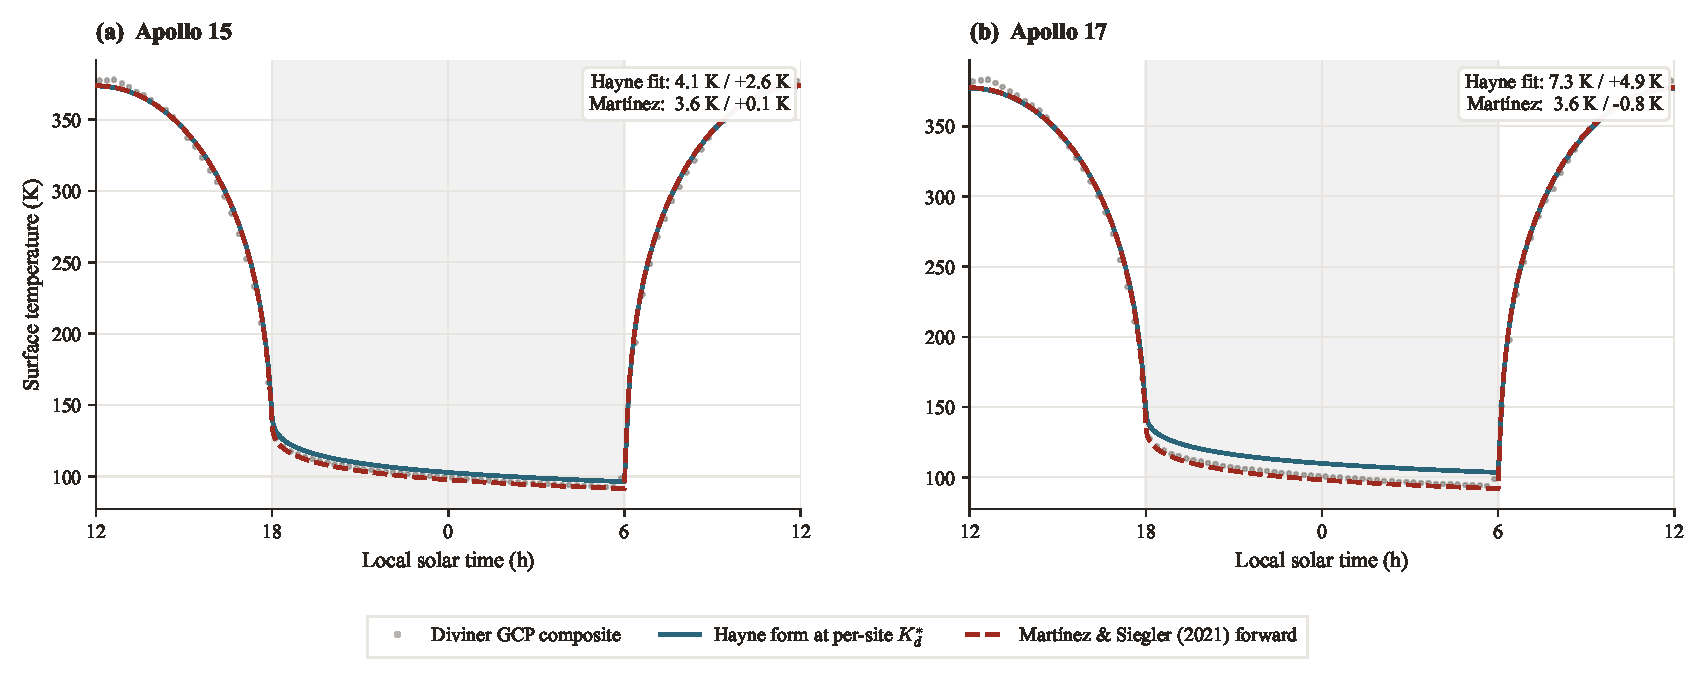
\includegraphics[width=\linewidth]{figures/fig_diviner_closure.pdf}\end{minipage}\hfill
\begin{minipage}{0.49\linewidth}\centering
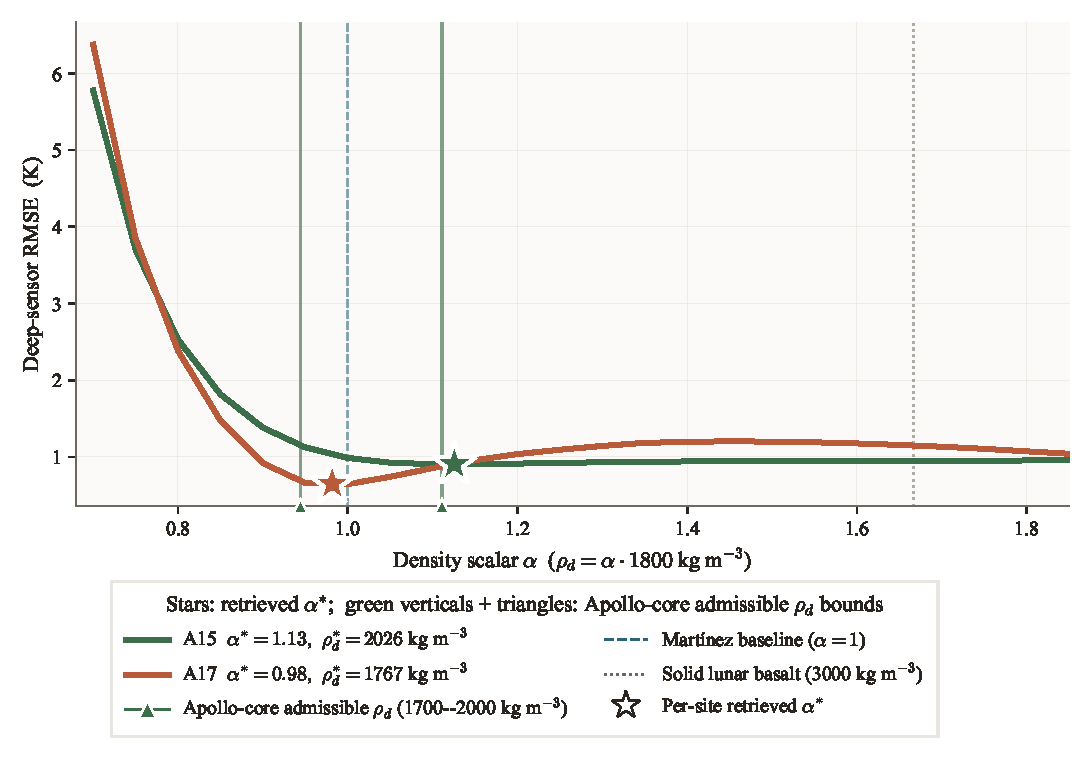
\includegraphics[width=\linewidth]{figures/fig_alpha_sweep.pdf}\end{minipage}
\caption{Left: the model with the retrieved $K_d$ reproduces the Diviner surface
temperatures. Right: the Mart\'inez density retrieval tells the same story.}
\label{fig:diviner}\label{fig:alpha}
\end{figure}

% =====================================================================
\chapter{How the code is organised, and a C++ future}\label{ch:code}
% =====================================================================
The code is layered (Fig.~\ref{fig:arch}): a physics package \code{lunar/} (the
models, grid, solver, equilibrium), thin driver scripts \code{scripts/}, and the
documents. One function, \code{run\_with}, is the hub everything calls.

\begin{figure}[h]\centering

\includegraphics[width=0.82\linewidth]{figures/fig_architecture.pdf}
\caption{Three layers; imports point only downward. The numerics live in three
small modules (\code{grid}, \code{solver}, \code{equilibrium}).}
\label{fig:arch}
\end{figure}

\paragraph{C++ port.} The time is spent in the inner step (\S\ref{ch:solver}),
run hundreds of thousands of times. The tridiagonal solve is already
JIT-compiled; the matrix assembly is interpreted Python --- exactly where a
compiled language wins ($\sim$10--100$\times$). The plan: port \code{grid},
\code{solver}, \code{equilibrium} to C++, keep configuration and analysis in
Python, and validate the port against the existing 37-test suite and the
committed steady-state profiles. The three speed-ups multiply: the algorithm (the
shortcut, $\sim$30$\times$, done) $\times$ compilation $\times$ parallel
independent solves. Not needed for this paper; valuable at scale.

% =====================================================================
\chapter{Conclusion: how to defend every claim}\label{ch:conclusion}
% =====================================================================
\begin{itemize}[leftmargin=1.5em,itemsep=3pt]
\item \textbf{What we did.} Retrieved the deep regolith conductivity separately at
Apollo~15 and~17: $4.58$ and $8.12$ mW\,m$^{-1}$\,K$^{-1}$.
\item \textbf{How.} A 1-D heat model (Ch.~\ref{ch:physics}--\ref{ch:solver}) with
the Hayne conductivity (Ch.~\ref{ch:models}), solved to a certified steady state
(Ch.~\ref{ch:steady}), with $K_d$ chosen to minimise the deep-sensor misfit
(Ch.~\ref{ch:retrieval}).
\item \textbf{Why it's right.} The solver is unique by construction, certifies its
own convergence, is guess-independent, and is confirmed by brute force converging
onto it (\S\ref{sec:agree}); the result is statistically significant
(Ch.~\ref{ch:stats}) and echoed by an independent model (Ch.~\ref{ch:crosschecks}).
\item \textbf{The honest caveat.} $K_d$ is conditional on the assumed $Q_b$
(Ch.~\ref{ch:qb}); the robust statement is the inter-site \emph{direction}.
\item \textbf{The physics.} Apollo~17's deep regolith conducts heat about twice as
efficiently --- plausibly denser/more compacted/more rock-rich material
(Ch.~\ref{ch:sites}).
\end{itemize}

\vspace{4pt}
\noindent\textit{Reproduce everything:} \code{make retrieve} (the result),
\code{notebooks/equilibrium\_demo.ipynb} (old vs.\ new), and
\code{pytest tests/test\_equilibrium.py} (the certification). The animations
\code{spinup.gif}, \code{newmethod.gif}, \code{reconstruct.gif} accompany
Chapters~\ref{ch:steady}.

\end{document}
